\section{Appendix: Additional Experiments and Ablations}
\label{app:additional-experiments}

\begin{table}[h]
\centering
\footnotesize
\setlength{\tabcolsep}{4.5pt}
\caption{\textbf{Capability coverage.} No prior method spans both the causal and inference directions for arbitrary DAGs; StructFlow unifies them (and additionally provides an automated compiler and both static/dynamic conditioning, discussed in the text). \cmark~= supported, \xmark~= not supported. ``Explaining-away'' denotes capturing the denser posterior dependencies (moralization) induced at colliders; ``Exact density'' denotes evaluation of model likelihoods by change of variables. $^\dagger$DCM does not provide density evaluation as published; we note that a diffusion model \emph{does} admit exact likelihoods via its probability-flow ODE \citep{song2021scorebased}---which is precisely the continuous-time flow of the last column, and is the sense in which the two rightmost capabilities are not independent (see text).}
\label{tab:capability}
\begin{tabular}{l cccccc}
\toprule
& \rotatebox{90}{Arbitrary DAG~}
& \rotatebox{90}{Causal queries~}
& \rotatebox{90}{Amortized inference~}
& \rotatebox{90}{Explaining-away~}
& \rotatebox{90}{Exact density~}
& \rotatebox{90}{Continuous-time~} \\
\midrule
CAREFL \citep{khemakhem2021causal}              & \cmark & \cmark & \xmark & \xmark & \cmark & \xmark \\
Causal NF \citep{javaloy2023causal}             & \cmark & \cmark & \xmark & \xmark & \cmark & \xmark \\
StrNN \citep{chen2023structured}                & \cmark & \cmark & \xmark & \xmark & \cmark & \xmark \\
DCM \citep{chao2023interventional}              & \cmark & \cmark & \xmark & \xmark & \xmark$^\dagger$ & \xmark \\
Weilbach et al.\ \citep{weilbach2020structured} & \cmark & \xmark & \cmark & \cmark & \cmark & \cmark \\
Zhai et al.\ \citep{jeong_conditional_2025}     & \xmark & \xmark & \cmark & \xmark & \cmark & \cmark \\
\midrule
\textbf{StructFlow (ours)}                       & \cmark & \cmark & \cmark & \cmark & \cmark & \cmark \\
\bottomrule
\end{tabular}
\end{table}


\subsection{MNIST}

We additionally evaluate on MNIST digit generation with the simple two-node structure \texttt{labels}$\to$\texttt{images}, a sanity check at higher dimensionality (784 pixels vs.\ 4 scalar variables in the synthetic PGMs).

\rev{\paragraph{Discrete labels in a continuous flow.} The label block is embedded as a one-hot vector in $\mathbb{R}^{10}$ (standardized by the same mean/variance normalizer as every block; no dequantization noise is added). The flow-matching objective is well-defined for such discrete targets: the linear interpolant $y_t = (1-t)\varepsilon + t\,y_1$ has a density for every $t < 1$ even when $y_1$ is drawn from a mixture of point masses, so the regression target exists almost everywhere and the learned transport concentrates its mass near the one-hot vertices. Sampled labels are decoded by $\arg\max$, and conditioning on a label clamps its (normalized) one-hot block. The colored-MNIST digit variable receives the identical treatment (its color variable, by contrast, is genuinely continuous: a palette color plus Gaussian jitter).}

\paragraph{Results.} All flow-based methods successfully learn the joint and marginal distributions (Figure~\ref{fig:mnist-swd}, Appendix~\ref{app:results}), but dynamic conditioning exhibits notably higher SWD on the conditional $p(\text{images}|\text{labels})$ despite accurately representing the joint. This is a genuine distributional gap rather than an outlier artifact (full diagnostic in Appendix~\ref{app:results}): inspecting samples shows dynamic conditioning produces \emph{perceptually crisp} digits that occasionally render the \emph{wrong class} for the conditioning label---a broadly-distributed conditional error that raises SWD while leaving individual samples realistic. Section~\ref{sec:chain-stiffness} isolates the mechanism behind this gap: dynamic conditioning's clamped condition trajectories leave the training distribution as evidence becomes higher-dimensional and more informative, an error that solver effort does not repair.


\subsection{When Does Structure Help? A Sample-Efficiency Study}
\label{sec:sample-efficiency}

The ablation above shows that the \emph{right} structure (with the co-parent edge) is necessary for correctness. A complementary question is when sparsity is an \emph{advantage}. On the small, well-sampled PGMs of Figure~\ref{fig:inference-nonlinear-pgm}, an unstructured flow can match a structured one because it has enough data to fit its extra (spurious) dependencies harmlessly. Structure should matter most when data are scarce, where its hard sparsity acts as an inductive bias that reduces variance.

We test this on a linear-Gaussian chain $x_0 \to x_1 \to \cdots \to x_5$, inferring $p(x_0,\dots,x_4 \mid x_5)$ (the exact posterior is Gaussian). We compare two static flows of the same family that differ only in connectivity: the \textbf{sparse} structure produced by our compiler ($5$ edges) and a \textbf{dense}, fully-connected flow ($15$ edges). Both are trained identically across a range of training-set sizes $N$, and we measure the $2$-Wasserstein distance between each flow's posterior and the exact posterior---an interpretable, zero-based metric.

Figure~\ref{fig:sample-efficiency} shows the result. The structured (sparse) flow is more accurate at every $N$, and the gap is largest in the low-data regime ($1.9\times$ lower error at $N{=}64$), narrowing as $N$ grows and the dense flow accumulates enough data to suppress its spurious dependencies. This is the expected behaviour of a correct inductive bias, and it explains the comparable performance of structured and unstructured flows in the well-sampled setting of Figure~\ref{fig:inference-nonlinear-pgm}: structure is most valuable precisely when data are limited. We present this single linear-Gaussian chain---which isolates the mechanism against an exact Gaussian posterior---as an illustration of the bias--variance trade-off that hard sparsity induces, not as a quantitative law; the magnitude of the advantage will depend on graph density and dimensionality.

\begin{figure}[t]
    \centering
    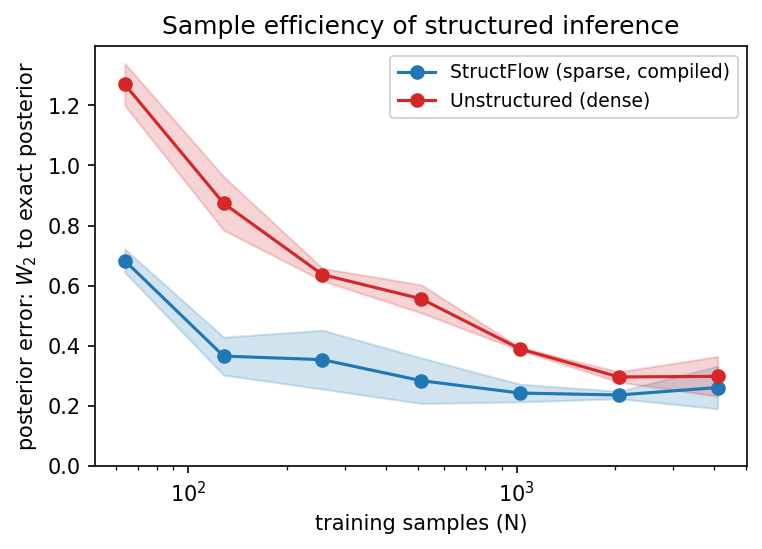
\includegraphics[width=0.55\columnwidth]{images/ablations/sample_efficiency.png}
    \caption{\textbf{Structure as an inductive bias.} Posterior error ($2$-Wasserstein to the exact posterior) versus training-set size for a linear-Gaussian chain: the compiler's sparse structure (blue) outperforms an unstructured dense flow (red) of the same family, with the largest advantage when data are scarce; the two converge as $N$ grows (bands: $\pm 1$ s.d.\ over seeds).}
    \label{fig:sample-efficiency}
\end{figure}

\subsection{Ablation: Does the Backbone Matter?}
\label{sec:backbone-ablation}

The comparisons above vary the \emph{structure} while holding the backbone fixed. Because
diffusion models and flow matching are the same object class up to reparameterization
(Section~\ref{par:backbone}), the complementary experiment is to vary the backbone while
holding the structure fixed. We therefore replace each block's continuous-time velocity field
with a per-node denoising diffusion model conditioned on the block's parents---the
construction of DCM \citep{chao2023interventional} and Diff-SCM
\citep{sanchez2022diffusion}---and re-run causal alignment on the same graphs, the same data,
and a matched parameter budget. Abduction uses DDIM inversion, as in those works. We present
this as an \emph{ablation of our own framework}, not as a competitor comparison: the question
is whether the compiler or the backbone is load-bearing.

Proposition~\ref{prop:abduction-error} makes a falsifiable prediction. Interventional queries
require no inversion, so the two backbones should agree; counterfactual queries require
abduction, where the CNF's error is solver tolerance at fixed weights while DDIM inversion
carries a first-order term in the step size. We therefore report accuracy as a function of
sampling compute (number of function evaluations, NFE) rather than at a single operating
point, since a single-NFE comparison cannot distinguish a backbone difference from a budget
choice.

Figure~\ref{fig:backbone-nfe} shows the result on the nonlinear $4$-node benchmark (5 PGM seeds, matched parameter budgets, NFE counted as \emph{network evaluations} per sample---RK4 costs four per step, DDIM one---so the axis is compute, not step count). Three observations. \emph{Interventional queries}: the backbones agree at moderate-to-high NFE (${\geq}16$; SWD $0.023$--$0.025$), with the diffusion variant degrading below that because its forward sampler is itself first-order, while the CNF remains flat even at a single RK4 step. \emph{Abduction error}---the direct measurement of Proposition~\ref{prop:abduction-error}---separates the backbones cleanly: the diffusion variant's reconstruction error $\lVert \mathrm{invert}(\mathrm{forward}(u)) - u \rVert$ decays at almost exactly first order in NFE (halving per doubling), exactly as predicted for published DDIM inversion, while the CNF's decays at roughly second order and ends ${\sim}55\times$ lower at NFE $128$. \emph{Counterfactual SWD} rises $10\times$ for the diffusion backbone as NFE falls from $128$ to $4$, versus $2.4\times$ for the CNF; one honest nuance is that at NFE ${\geq}64$ the diffusion variant's counterfactual SWD is slightly \emph{below} the CNF's ($0.0047$ vs $0.0085$) despite its far larger pointwise abduction error---SWD is a distributional metric and does not penalize an inversion bias that approximately preserves the noise distribution, which is why the abduction panel, not the counterfactual panel, is the proposition's direct test. Finally, the inference-mode columns are empty for the diffusion backbone by construction: per-node diffusion supplies no amortized posterior, no moralization, and no conditional density (its NLL/KL entries correctly surface as unavailable). Training differs in one respect we could not match: the flow variants use minibatch OT coupling, which has no diffusion analogue.

\begin{figure*}[t]
    \centering
    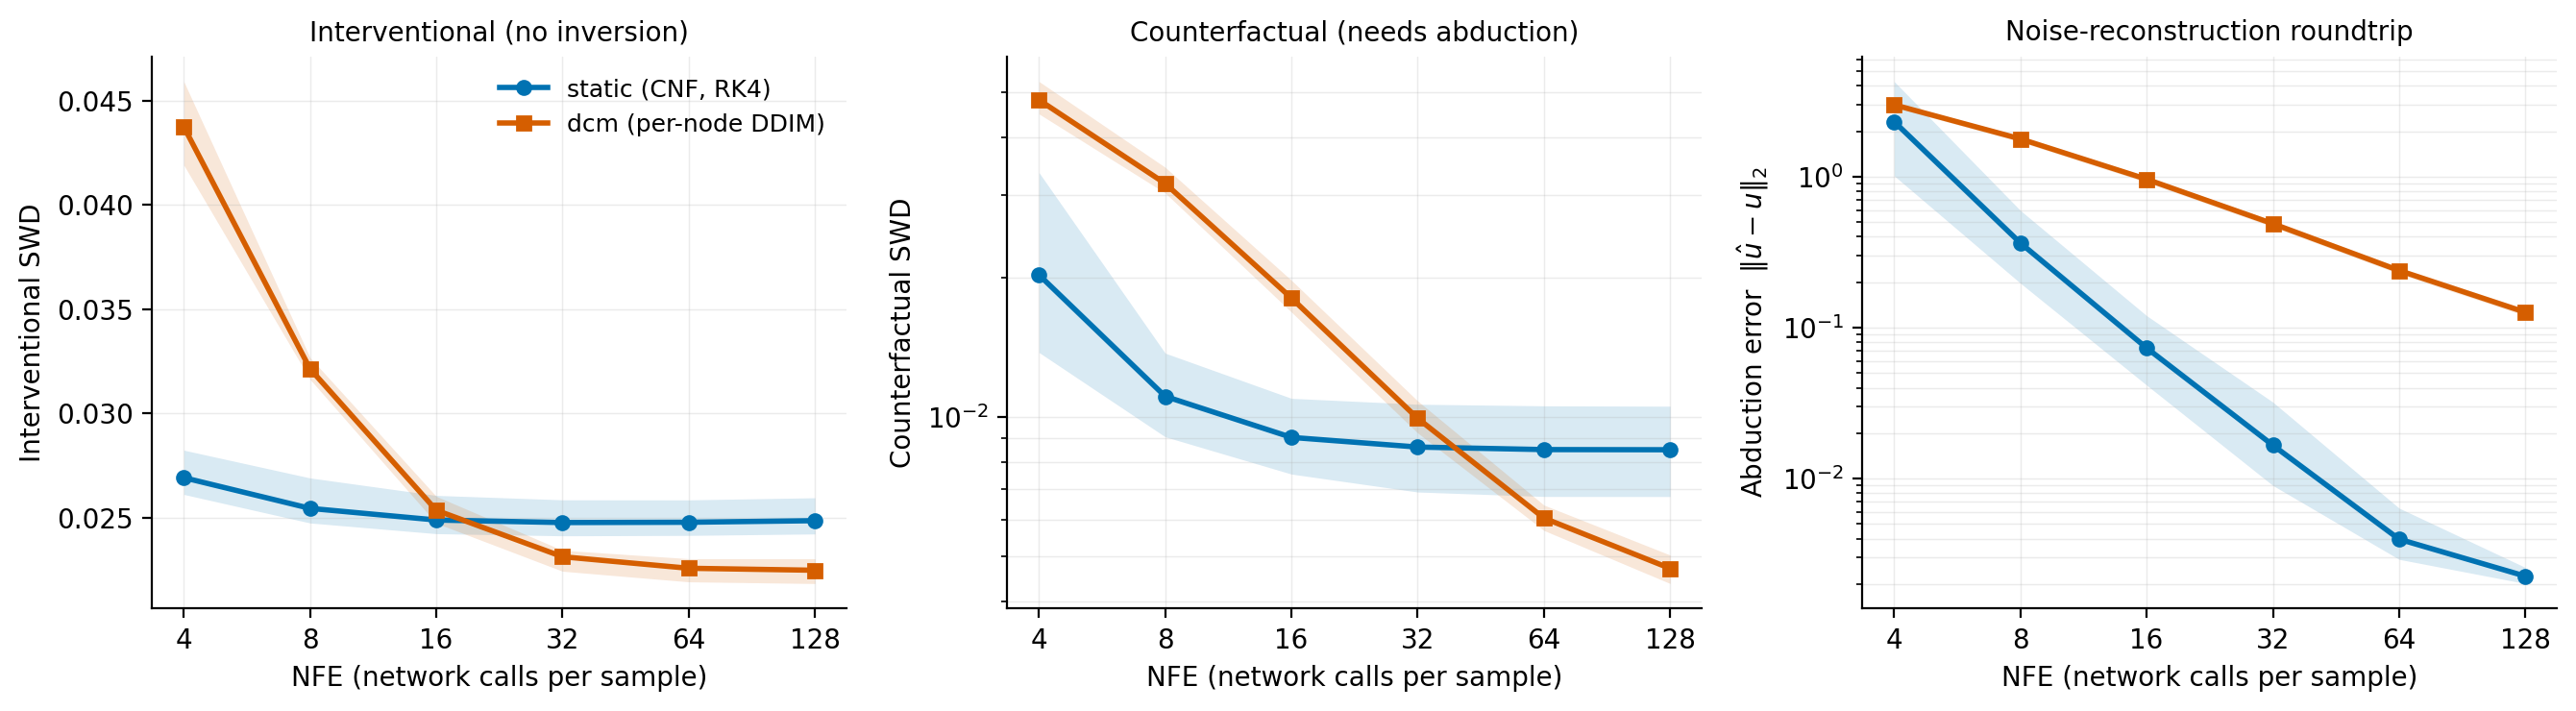
\includegraphics[width=\textwidth]{images/ablations/backbone_nfe.png}
    \caption{\textbf{Backbone ablation on nonlinear 4-node PGMs} (mean $\pm$ range over 5 PGM seeds; $x$-axis is measured network evaluations per sample). \textbf{Left:} interventional SWD---backbones agree for NFE $\geq 16$. \textbf{Middle:} counterfactual SWD---the diffusion backbone degrades far more steeply at low NFE. \textbf{Right:} abduction reconstruction error---first-order decay for DDIM inversion versus ${\sim}$second-order for the CNF, the direct measurement of Proposition~\ref{prop:abduction-error}.}
    \label{fig:backbone-nfe}
\end{figure*}

The outcome we expect makes the paper's argument better than a win would. If the two
backbones tie on interventional queries and the diffusion variant has no inference-mode
entries at all, that is direct evidence that the compiled structure---not the choice of
continuous-time generative model---is what delivers the capabilities of
Table~\ref{tab:capability}.


\subsection{Inference Alignment: Amortized Probabilistic Inference}

For Inference Alignment, we use StructFlow to ``invert'' the DAG---edges point from children to parents, with additional edges via moralization. This enables efficient sampling from posterior distributions $p(\text{parents} | \text{children})$.

\paragraph{Results.} Figure \ref{fig:inference-nonlinear-pgm} shows that our structured flows can effectively learn to perform probabilistic inference, providing accurate amortized inference over the model's latent variables. On these small, well-sampled nonlinear PGMs all methods perform comparably---including the unstructured \textit{Guided} baseline. This is expected rather than contradictory: the Guided flow places dependencies between \emph{all} variables, so it implicitly contains the moral edges that the posterior requires. The ablation in Section~\ref{sec:moralization-ablation} isolates this effect, showing that the relevant structural ingredient is exactly the moralization our compiler performs; and Section~\ref{sec:sample-efficiency} shows that the benefit of \emph{sparse} structure (over a dense, unstructured flow) emerges when training data are limited. The same qualitative picture holds on larger random $8$-node nonlinear PGMs, confirming the framework is not limited to very small graphs (Appendix~\ref{app:results}, Figure~\ref{fig:inference-n8}); the binding constraint on scaling further is \emph{evaluation}---generating MCMC ground truth for every conditional query (Section~\ref{sec:future_work})---not training.

\subsection{Ablation: Is Moralization Necessary?}
\label{sec:moralization-ablation}

\rev{The compiled inference structure contains a dependency between the parents of a collider (the ``moral'' edge, produced by the d-separation step under the compiled ordering) to capture the posterior dependencies induced by ``explaining away''.} We test whether this edge is truly necessary on a linear-Gaussian collider $A \to C \leftarrow B$ with $A, B \sim \mathcal{N}(0,1)$ and $C = A + B + \sigma \epsilon$. Observing $C$ induces a strong negative correlation between $A$ and $B$, and the exact posterior $p(A, B \mid C)$ is available in closed form.

We compile the inference flow for the query $p(A, B \mid C)$ and compare the StructFlow architecture (which adds the moral edge $A\!-\!B$) against an ablated architecture with that edge removed---so the flow is forced to factorize as $p(A \mid C)\,p(B \mid C)$. Both are trained identically on the same joint samples.

Figure~\ref{fig:moralization-ablation} shows the outcome. The ablated (non-moralized) flow recovers the correct posterior \emph{marginals} but is structurally incapable of representing the posterior correlation, yielding $\mathrm{corr}(A, B \mid C) \approx 0$. The moralized StructFlow recovers it closely ($-0.94$ vs.\ the analytic $-0.92$; the small overshoot is within the seed-to-seed variation of the learned flow). \rev{This isolates the contribution of the compiled co-parent dependency: it is not a heuristic convenience but a requirement for faithfully representing collider posteriors.} We demonstrate the effect on this canonical collider because it admits a closed-form posterior, but the conclusion is \emph{structural} rather than specific to this instance: without an edge between two colliding parents, a block-triangular flow has no computational path to couple them, so it cannot represent any induced posterior correlation regardless of the underlying mechanism.

\begin{figure}[t]
    \centering
    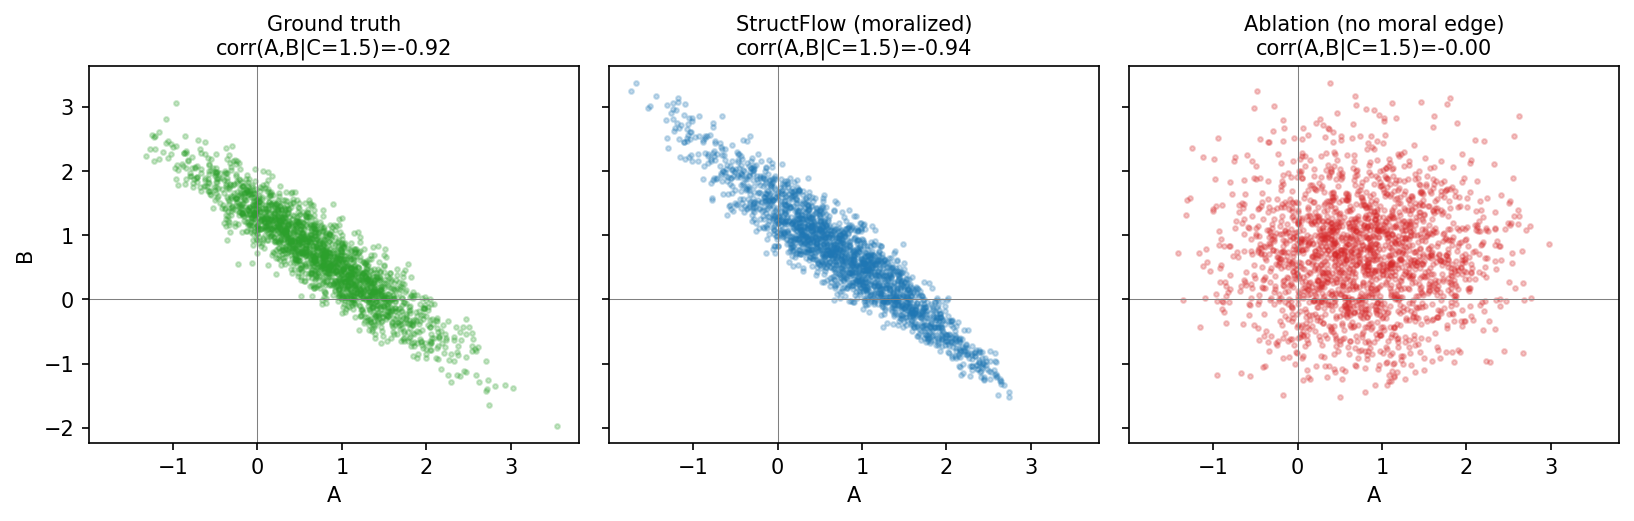
\includegraphics[width=0.82\columnwidth]{images/ablations/moralization_collider.png}
    \caption{\textbf{The compiled co-parent dependency is necessary for explaining-away.} Posterior samples of $p(A, B \mid C{=}1.5)$ for the collider $A \to C \leftarrow B$. \textbf{Left:} analytic ground truth (strong negative correlation). \textbf{Middle:} StructFlow with the moral edge recovers the correlation. \textbf{Right:} the ablation without the moral edge captures the marginals but collapses the correlation to $\approx 0$.}
    \label{fig:moralization-ablation}
\end{figure}

\subsection{Ablation: Separating Moralization from d-Separation}
\label{app:ordering-ablation}
\rev{
The compiler's two graph-processing steps play different roles, and this ablation separates them. The dependency set of a compiled structure is constructed \emph{entirely} by the d-separation step: for any ordering with the conditions as a prefix, each block's parents are exactly the predecessors it is not d-separated from in the original DAG. Moralization enters only through the breadth-first traversal that \emph{chooses} the ordering---marrying co-parents so that explaining-away partners are visited adjacently. We therefore compile the leaf-conditioned posterior of each test graph under three ordering policies, holding the d-separation step fixed: (a)~the moral-BFS ordering (the compiler as shipped), (b)~a no-moralization ordering (conditions first, remaining variables in reverse topological order), and (c)~$20$ random orderings with the conditions kept as a prefix.

Two findings. \emph{First, correctness never depends on the ordering policy}: on the collider of Section~\ref{sec:moralization-ablation}, the co-parent dependency appears in the compiled structure under \emph{every} ordering tested---it is forced by d-separation ($A \not\perp_d B \mid C$), so the posterior dependencies that Figure~\ref{fig:moralization-ablation} shows to be necessary are supplied by the d-separation step regardless of how the ordering was chosen. \emph{Second, the ordering policy controls sparsity}: across colliders, chains ($n \in \{4, 8\}$), and $15$ random DAGs ($n \in \{4, 6, 8\}$, five seeds each), the moral-BFS ordering never yields more compiled dependencies than the alternatives and yields strictly fewer on $11$ of $18$ graphs (mean $12.8$ edges vs.\ $13.9$ for the no-moralization ordering and $14.3$ for the random-order median; on the $8$-chain, adversarial orderings inflate $7$ edges to $13$). Since sparsity is the inductive bias behind the sample-efficiency results of Section~\ref{sec:sample-efficiency}, moralization earns its place as the ordering heuristic---but the compiled dependencies, and hence correctness, come from d-separation alone. The ablation is reproduced by \texttt{scripts/ablations/ordering\_ablation.py}.}

\subsection{Validating the NUTS References}
\label{app:nuts-validation}
\rev{
The nonlinear inference benchmarks are scored against NUTS reference posteriors, so their accuracy is load-bearing. The reference protocol draws each sample from an \emph{independent} chain (window adaptation for $250$ steps, then a single kept state, vectorized over chains), so the ensemble carries no autocorrelation but relies entirely on warmup convergence from a prior initialization---a failure of which would bias every chain identically and be invisible to within-chain diagnostics. We therefore validate the protocol three ways, on the benchmark graph family at both node dimensions used in the paper and at $n{=}16$ beyond it (\texttt{scripts/ablations/nuts\_validation.py}). \emph{Closed-form anchor}: on linear-Gaussian instances, where the exact posterior is available, the reference ensemble's Bures-$W_2$ to the analytic posterior is $2$--$4\%$ of the posterior scale at every benchmark size (up to $n{=}8$, $d{=}8$: $64$-dimensional joints), consistent with the finite-ensemble Monte-Carlo floor. \emph{Warmup sensitivity}: increasing warmup $4\times$ (and, at $n \le 8$, $16\times$) moves the ensemble by \emph{less} than its own resampling noise (SWD $0.030$--$0.074$ between warmup settings vs.\ half-split floors of $0.060$--$0.113$)---$250$ steps is converged. \emph{Simulation-based calibration} \citep{talts2018validating}: over $300$ replications per graph, ranking the joint draw among $99$ reference draws, the per-dimension $\chi^2$ uniformity $p$-values are consistent with uniform ranks on every benchmark-family graph (minimum $0.03$ across $40$ tested dimensions, as expected under uniformity). We conclude the reference error sits at the Monte-Carlo floor of the ensemble sizes used, well below the method differences the benchmarks measure.

The validation also has teeth: pushed beyond the benchmarks, to a \emph{linear} $n{=}16$, $d{=}8$ graph ($128$-dimensional joint), the protocol fails outright---anchor $W_2 \approx 52\times$ the posterior scale, SBC $p$-values below $10^{-13}$---because $16$ layers of random linear maps produce an ill-conditioned joint whose scale disparities defeat warmup adaptation from a prior initialization (diagnostically, ensembles at different warmup budgets agree with each other far better than either agrees with its own half-splits: the chains are frozen where they start). The nonlinear $n{=}16$ counterpart, whose spline mechanisms keep the joint well-conditioned, passes all checks. Accordingly, any linear-Gaussian evaluation at $n{=}16$ must use the closed-form conditionals rather than the MCMC reference path.}

\subsection{Amortized Inference vs.\ MCMC}
\label{sec:amortization}

A practical advantage of Inference Alignment is \emph{amortization}: the flow is trained once, after which any posterior query $p(\text{targets} \mid \text{conditions}{=}c)$ is answered with a single fast ODE solve, whereas a classical sampler such as the No-U-Turn Sampler (NUTS) must run a fresh Markov chain for every observed value $c$. On a nonlinear collider, Figure~\ref{fig:amortization} (right) confirms that StructFlow's amortized posterior and a NUTS reference agree closely (mean Sliced Wasserstein distance $0.0014$ across queries), while Figure~\ref{fig:amortization} (left) shows the wall-clock trade-off: StructFlow pays a one-time training cost but is roughly $11\times$ faster \emph{per query}, so its cumulative cost overtakes per-query MCMC after a crossover of $K^\star \approx 22$ queries. The specific speedup and crossover are setup-dependent (Appendix~\ref{app:experiments}), but the qualitative conclusion is general: structured amortized inference is preferable whenever many posterior queries must be answered for the same model.

\begin{figure}[t]
    \centering
    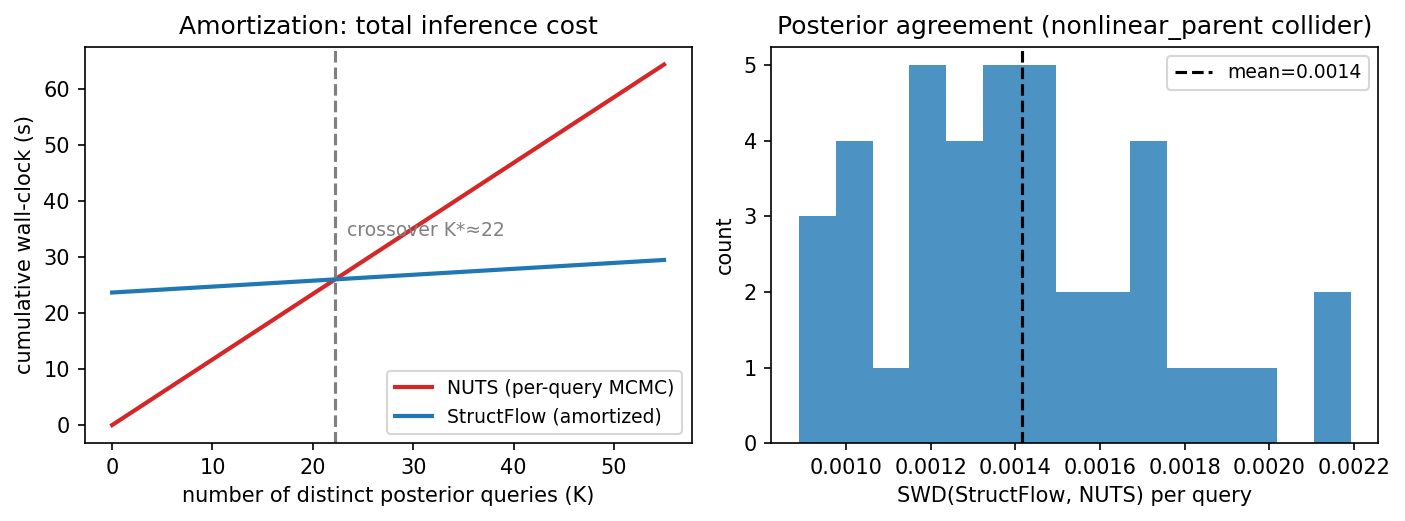
\includegraphics[width=0.95\columnwidth]{images/ablations/amortization_vs_nuts.png}
    \caption{\textbf{Amortized inference vs.\ per-query MCMC} on a nonlinear collider. Left: cumulative wall-clock versus the number of distinct posterior queries; the amortized flow overtakes NUTS after $K^\star \approx 22$ queries. Right: per-query agreement between StructFlow and the NUTS reference (Sliced Wasserstein distance).}
    \label{fig:amortization}
\end{figure}


\subsection{Colored-MNIST: Intervene-vs-Observe Heatmaps}

\begin{figure*}[t]
    \centering
    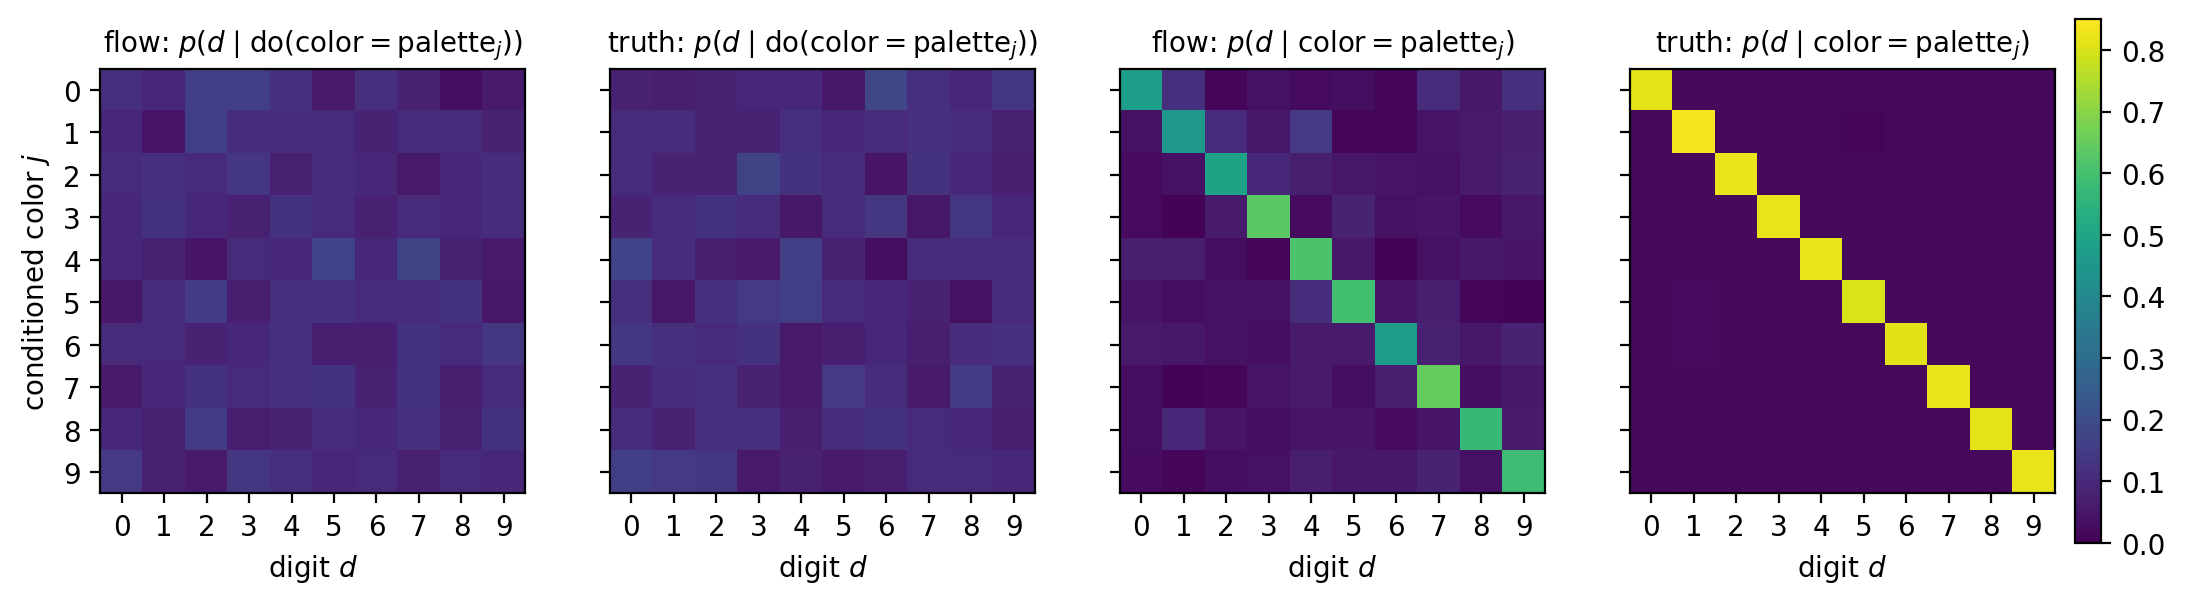
\includegraphics[width=\textwidth]{images/colored_mnist_conv_heatmaps.png}
    \caption{\textbf{Intervening vs.\ conditioning on Colored-MNIST.} Digit marginals for each conditioned palette color $j$ (rows). Under $\mathrm{do}(\mathrm{color})$ (left pair) the digit distribution is unchanged---both the flow and the sampled ground truth are uniform. Under observational conditioning (right pair) the posterior concentrates on the color-correlated digit: the flow (third panel) recovers the diagonal of the exact analytic posterior (fourth panel; noise-free because it is computed in closed form, whereas the truth-interventional panel is sampled).}
    \label{fig:colored-mnist-heatmaps}
\end{figure*}

\subsection{Colored-MNIST at $\rho = 1$: Zero-Shot Counterfactuals}
\label{app:colored-mnist-rho1}

\begin{figure}[t]
    \centering
    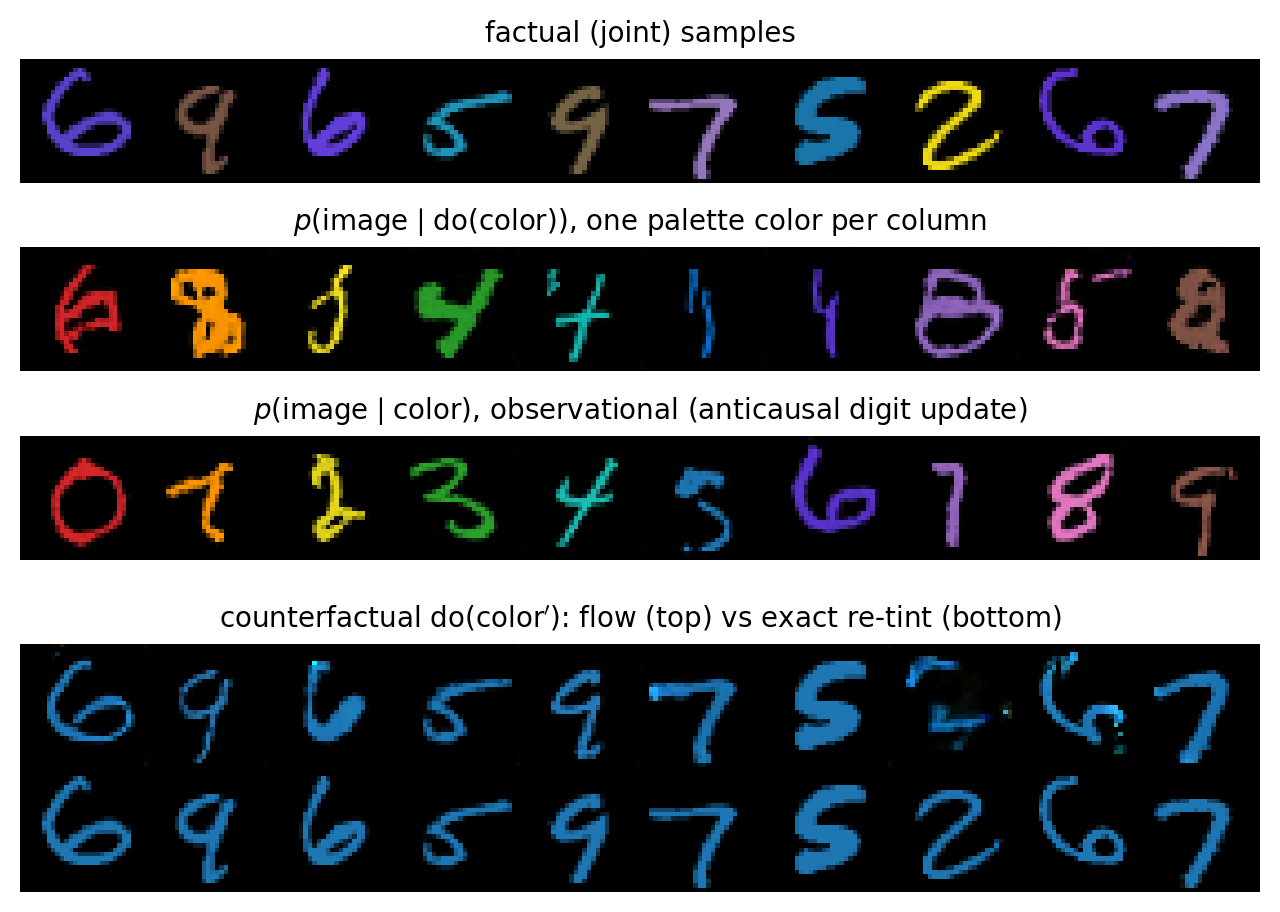
\includegraphics[width=0.6\columnwidth]{images/colored_mnist_rho1_strips.png}
    \caption{\textbf{Colored-MNIST with deterministic colors ($\rho = 1$).} Same layout as Figure~\ref{fig:colored-mnist-strips}, retrained on data where every digit always wears its palette color, so no off-diagonal (digit, color) pair ever appears in training. Row 2: interventional samples still extrapolate to every unseen combination. Row 3: the observational posterior is now a point mass, and the flow produces exactly one digit per color. Row 4: counterfactual re-coloring is now genuinely zero-shot mechanism transfer; most samples match the exact re-tint, and the failures (e.g.\ the thick `2') are abduction failures---inverting a factual image through a flow whose training support never dissociated digit from color.}
    \label{fig:colored-mnist-rho1}
\end{figure}
